\documentclass[]{article}
\usepackage{listings}
\usepackage{xcolor}
\usepackage{graphicx}
\usepackage{circuitikz}
\definecolor{codegreen}{HTML}{859900}
\definecolor{codegray}{HTML}{839496}
\definecolor{codepurple}{HTML}{6C71C4}
\definecolor{codemagenta}{HTML}{d33682}
\definecolor{backcolour}{HTML}{FDF6E3}
\definecolor{fontcolor}{HTML}{002B36}
\lstdefinestyle{mystyle}{
	basicstyle=\color{fontcolor},
	backgroundcolor=\color{backcolour},   
	commentstyle=\color{codegreen},
	keywordstyle=\color{codemagenta},
	numberstyle=\tiny\color{codegray},
	stringstyle=\color{codepurple},
	breakatwhitespace=false,         
	breaklines=true,                 
	captionpos=b,                    
	keepspaces=true,                 
	numbers=left,                    
	numbersep=5pt,                  
	showspaces=false,                
	showstringspaces=false,
	showtabs=false,                  
	tabsize=4
}
\lstset{style=mystyle}
\title{Lab 5\\Timers}
\author{Keaton Clark}

\begin{document}
\maketitle
\section*{Circuit}
	\begin{center}
		\begin{circuitikz}
			\draw (0,0) to 
				[short,l={$D_{12}$},o-](2,0) to 
				[loudspeaker](2,-2) to 
				(0,-2)node[ground]{}
			;
		\end{circuitikz}
	\end{center}
\section*{Data}
	\begin{center}
		\begin{tabular}{|c|c|c|}
			\hline
			Note & Target Frequency(Hz) & Measured Frequency(Hz)\\
			\hline
			A & 440 & 436.44\\
			\hline
			B & 494 & 489.49\\
			\hline
			C & 523 & 518.02\\
			\hline
			D & 587 & 580.76\\
			\hline
			E & 659 & 651.11\\
			\hline
			F & 698 & 689.14\\
			\hline
			G & 784 & 772.85\\
			\hline
		\end{tabular}
	\end{center}
\section*{Questions}
	\begin{enumerate}
		\item
			The measured frequency seems to seperate from the target frequency with an increasing margin. This could be due to the clock being slightly under 16Mhz and therefore being increasing more offset the more clock pulse we wait for.
	\end{enumerate}
\section*{Images}
	\begin{center}
		\pagebreak
		Note: A\\
		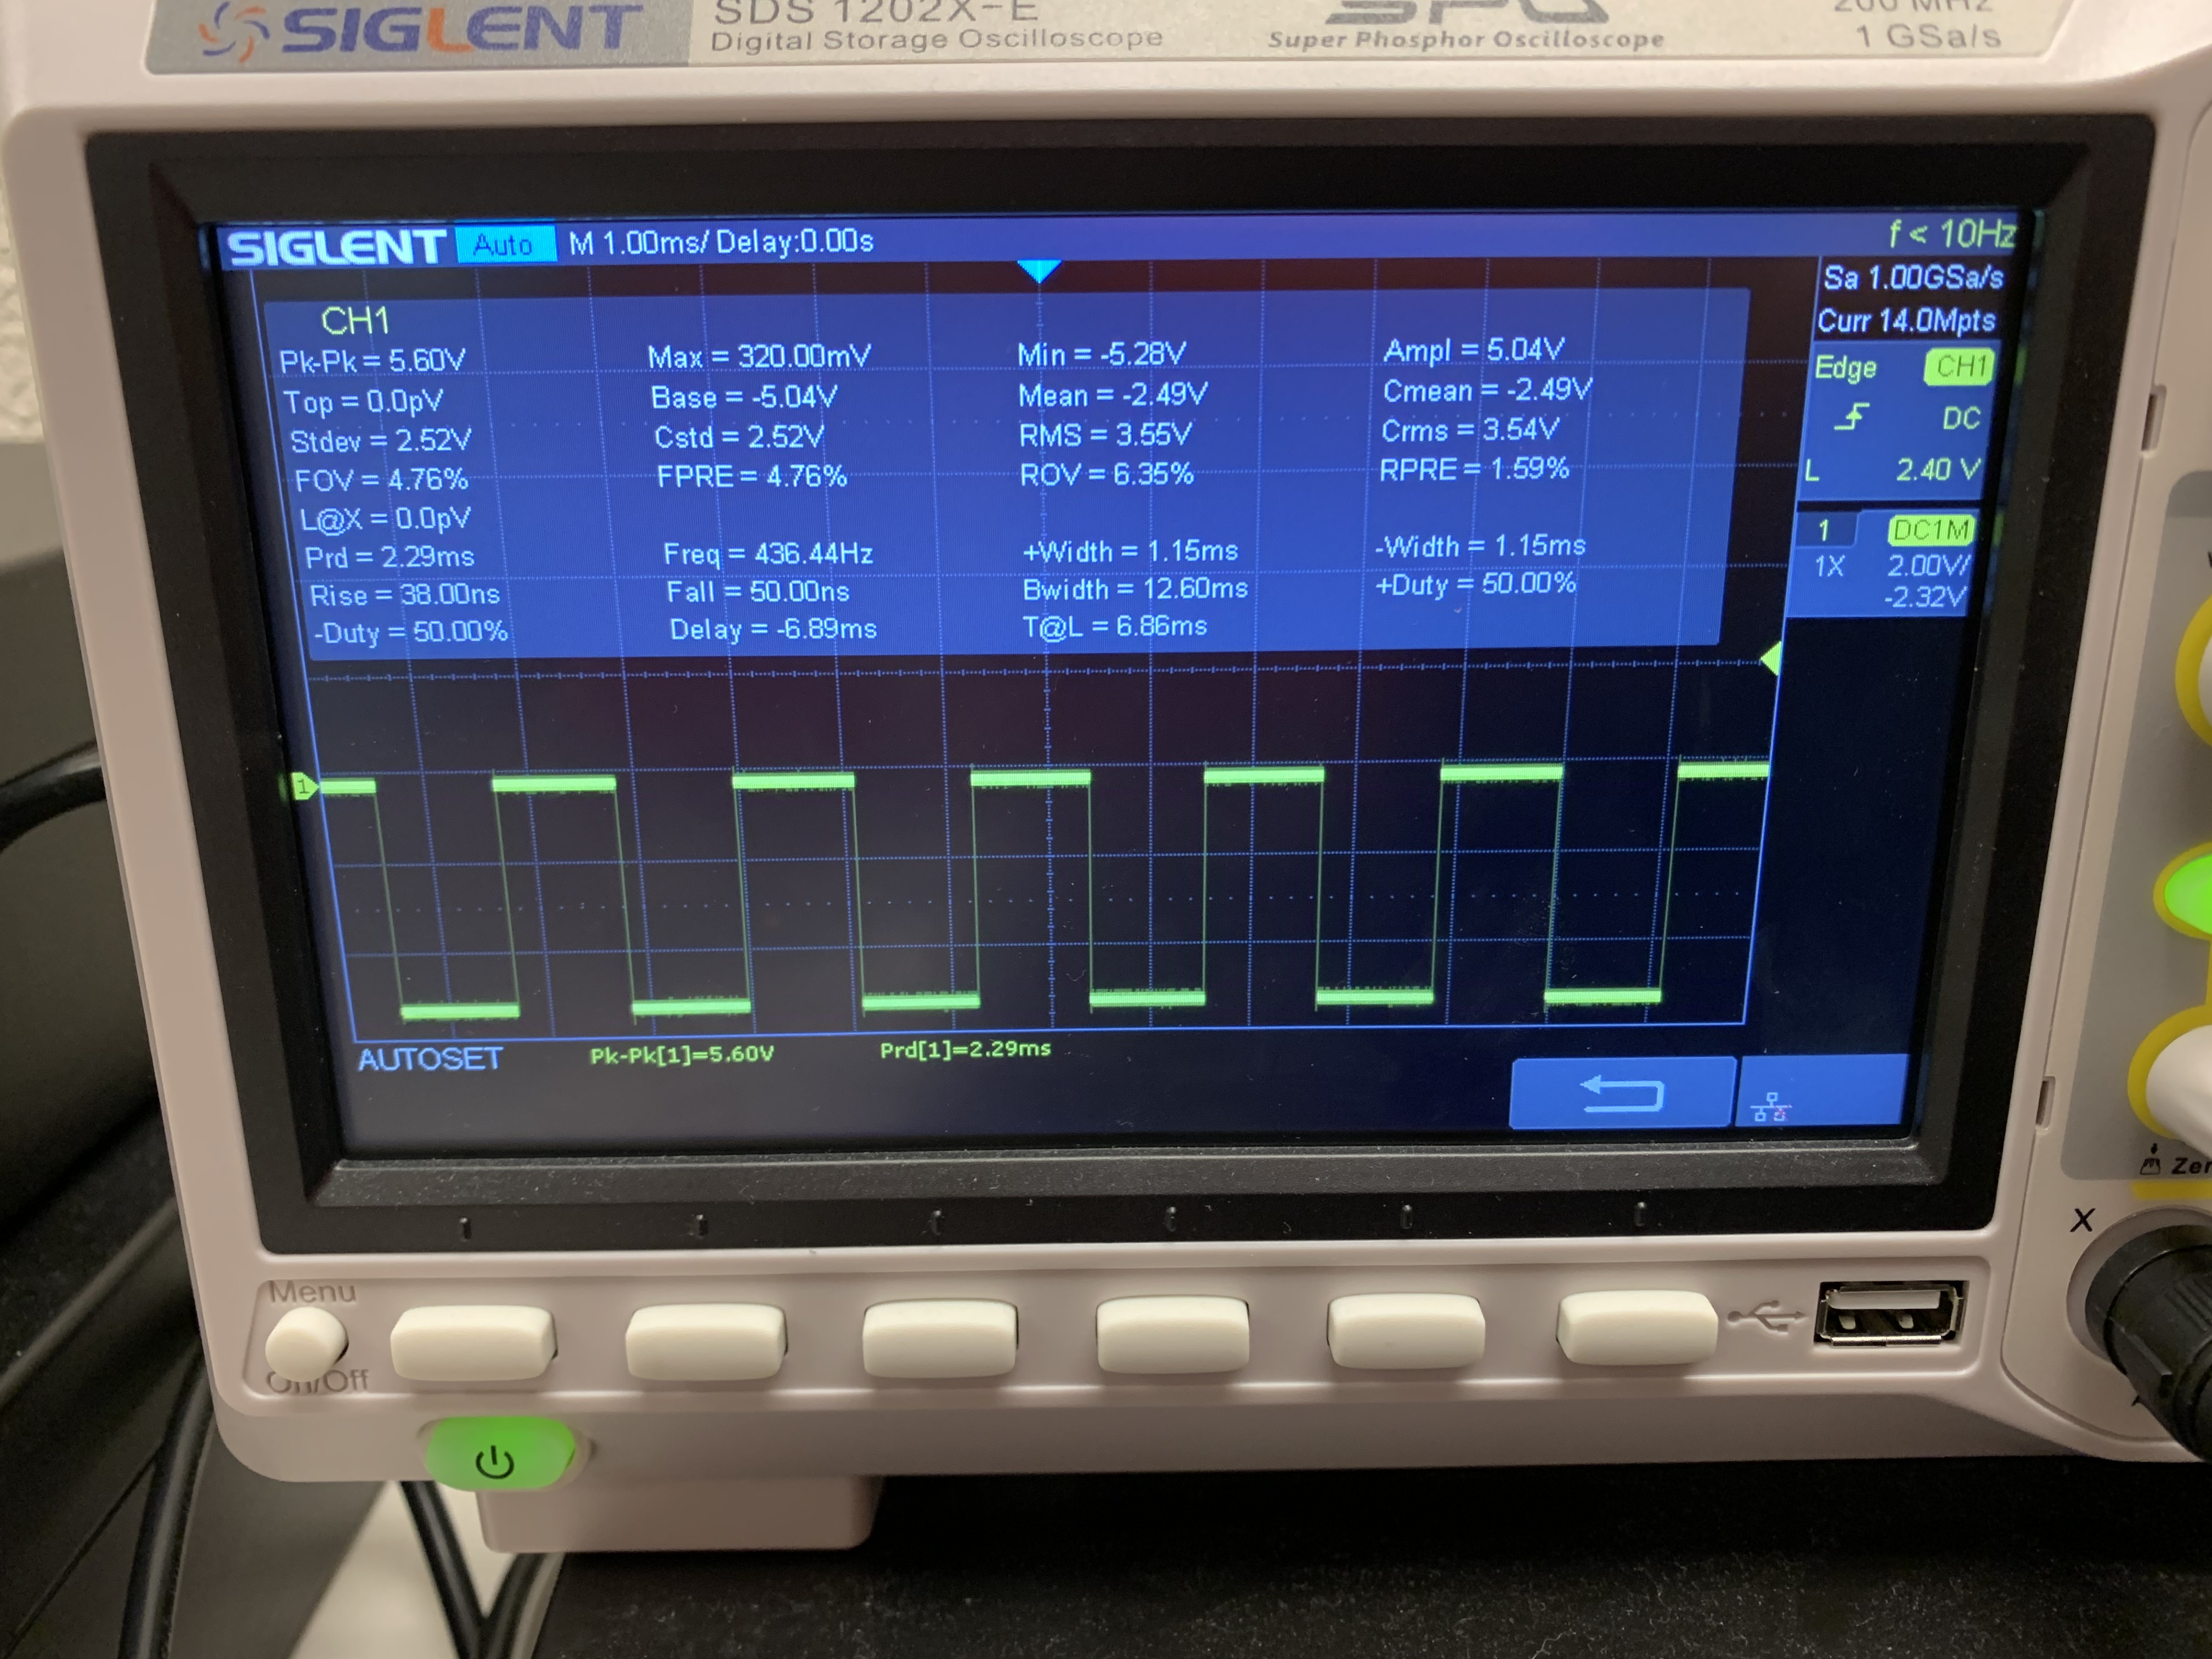
\includegraphics[scale=.05]{./images/0.jpg}\\
		Note: B\\
		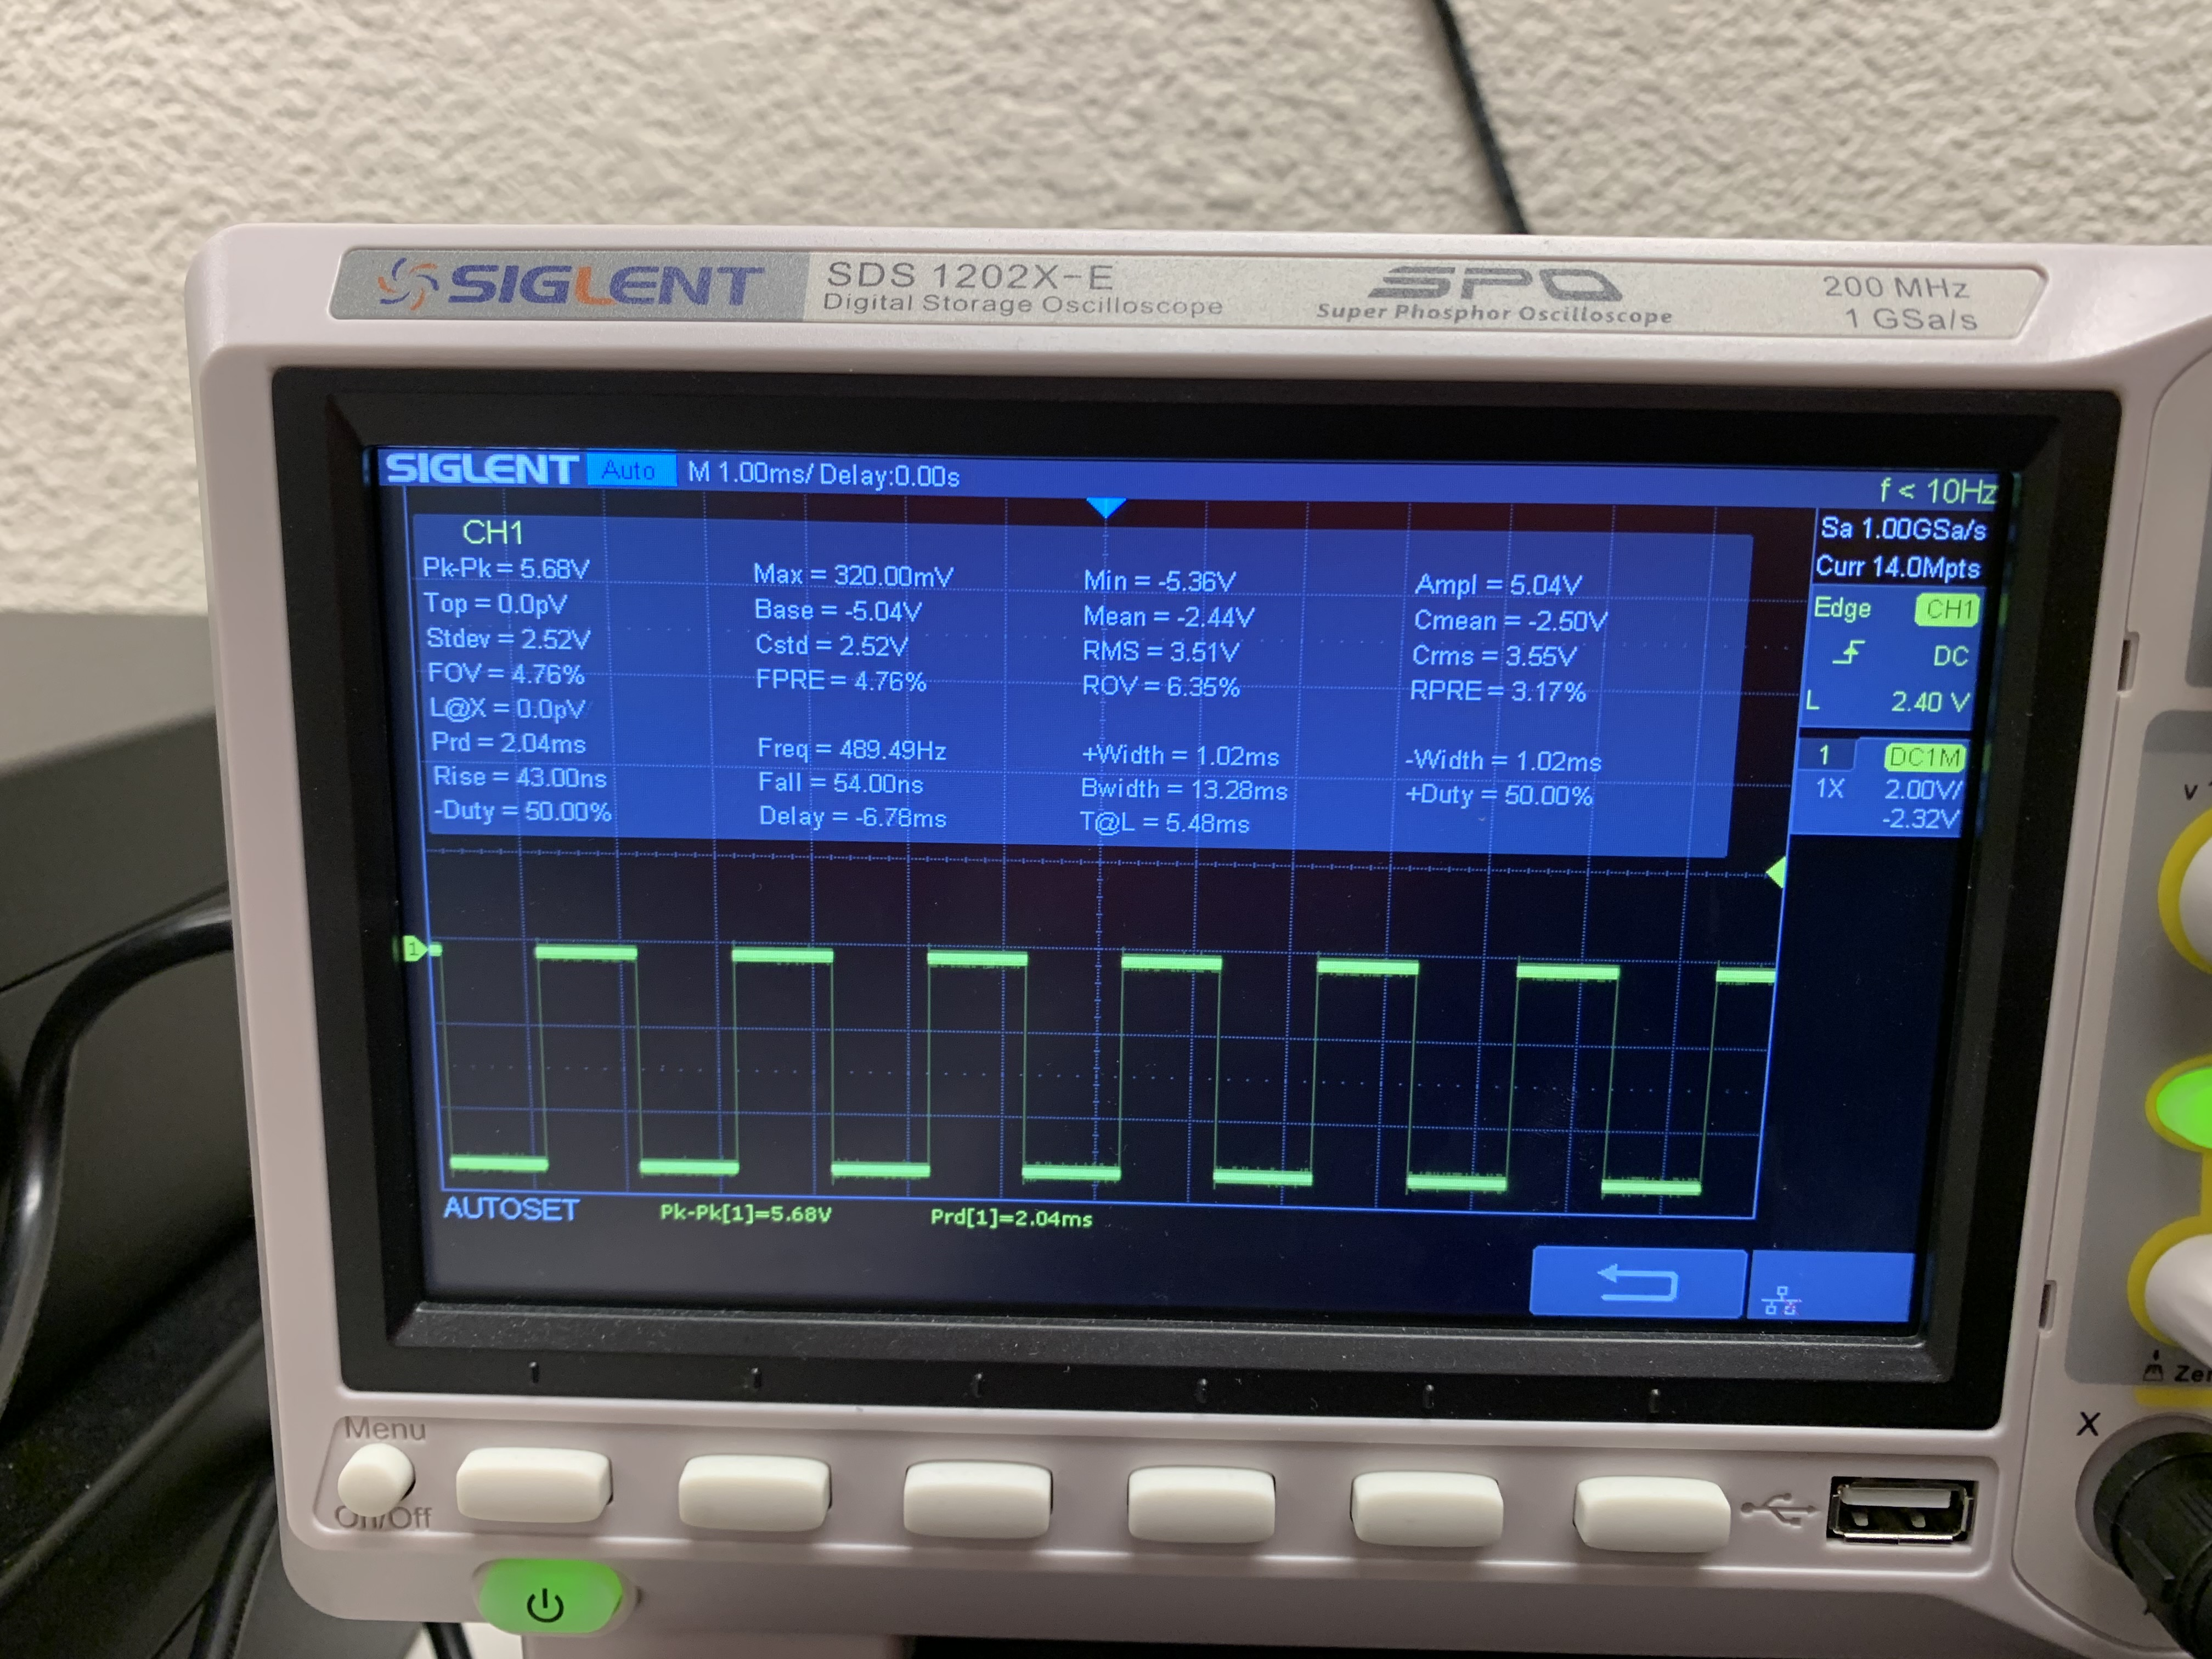
\includegraphics[scale=.05]{./images/1.jpg}\\
		Note: C\\
		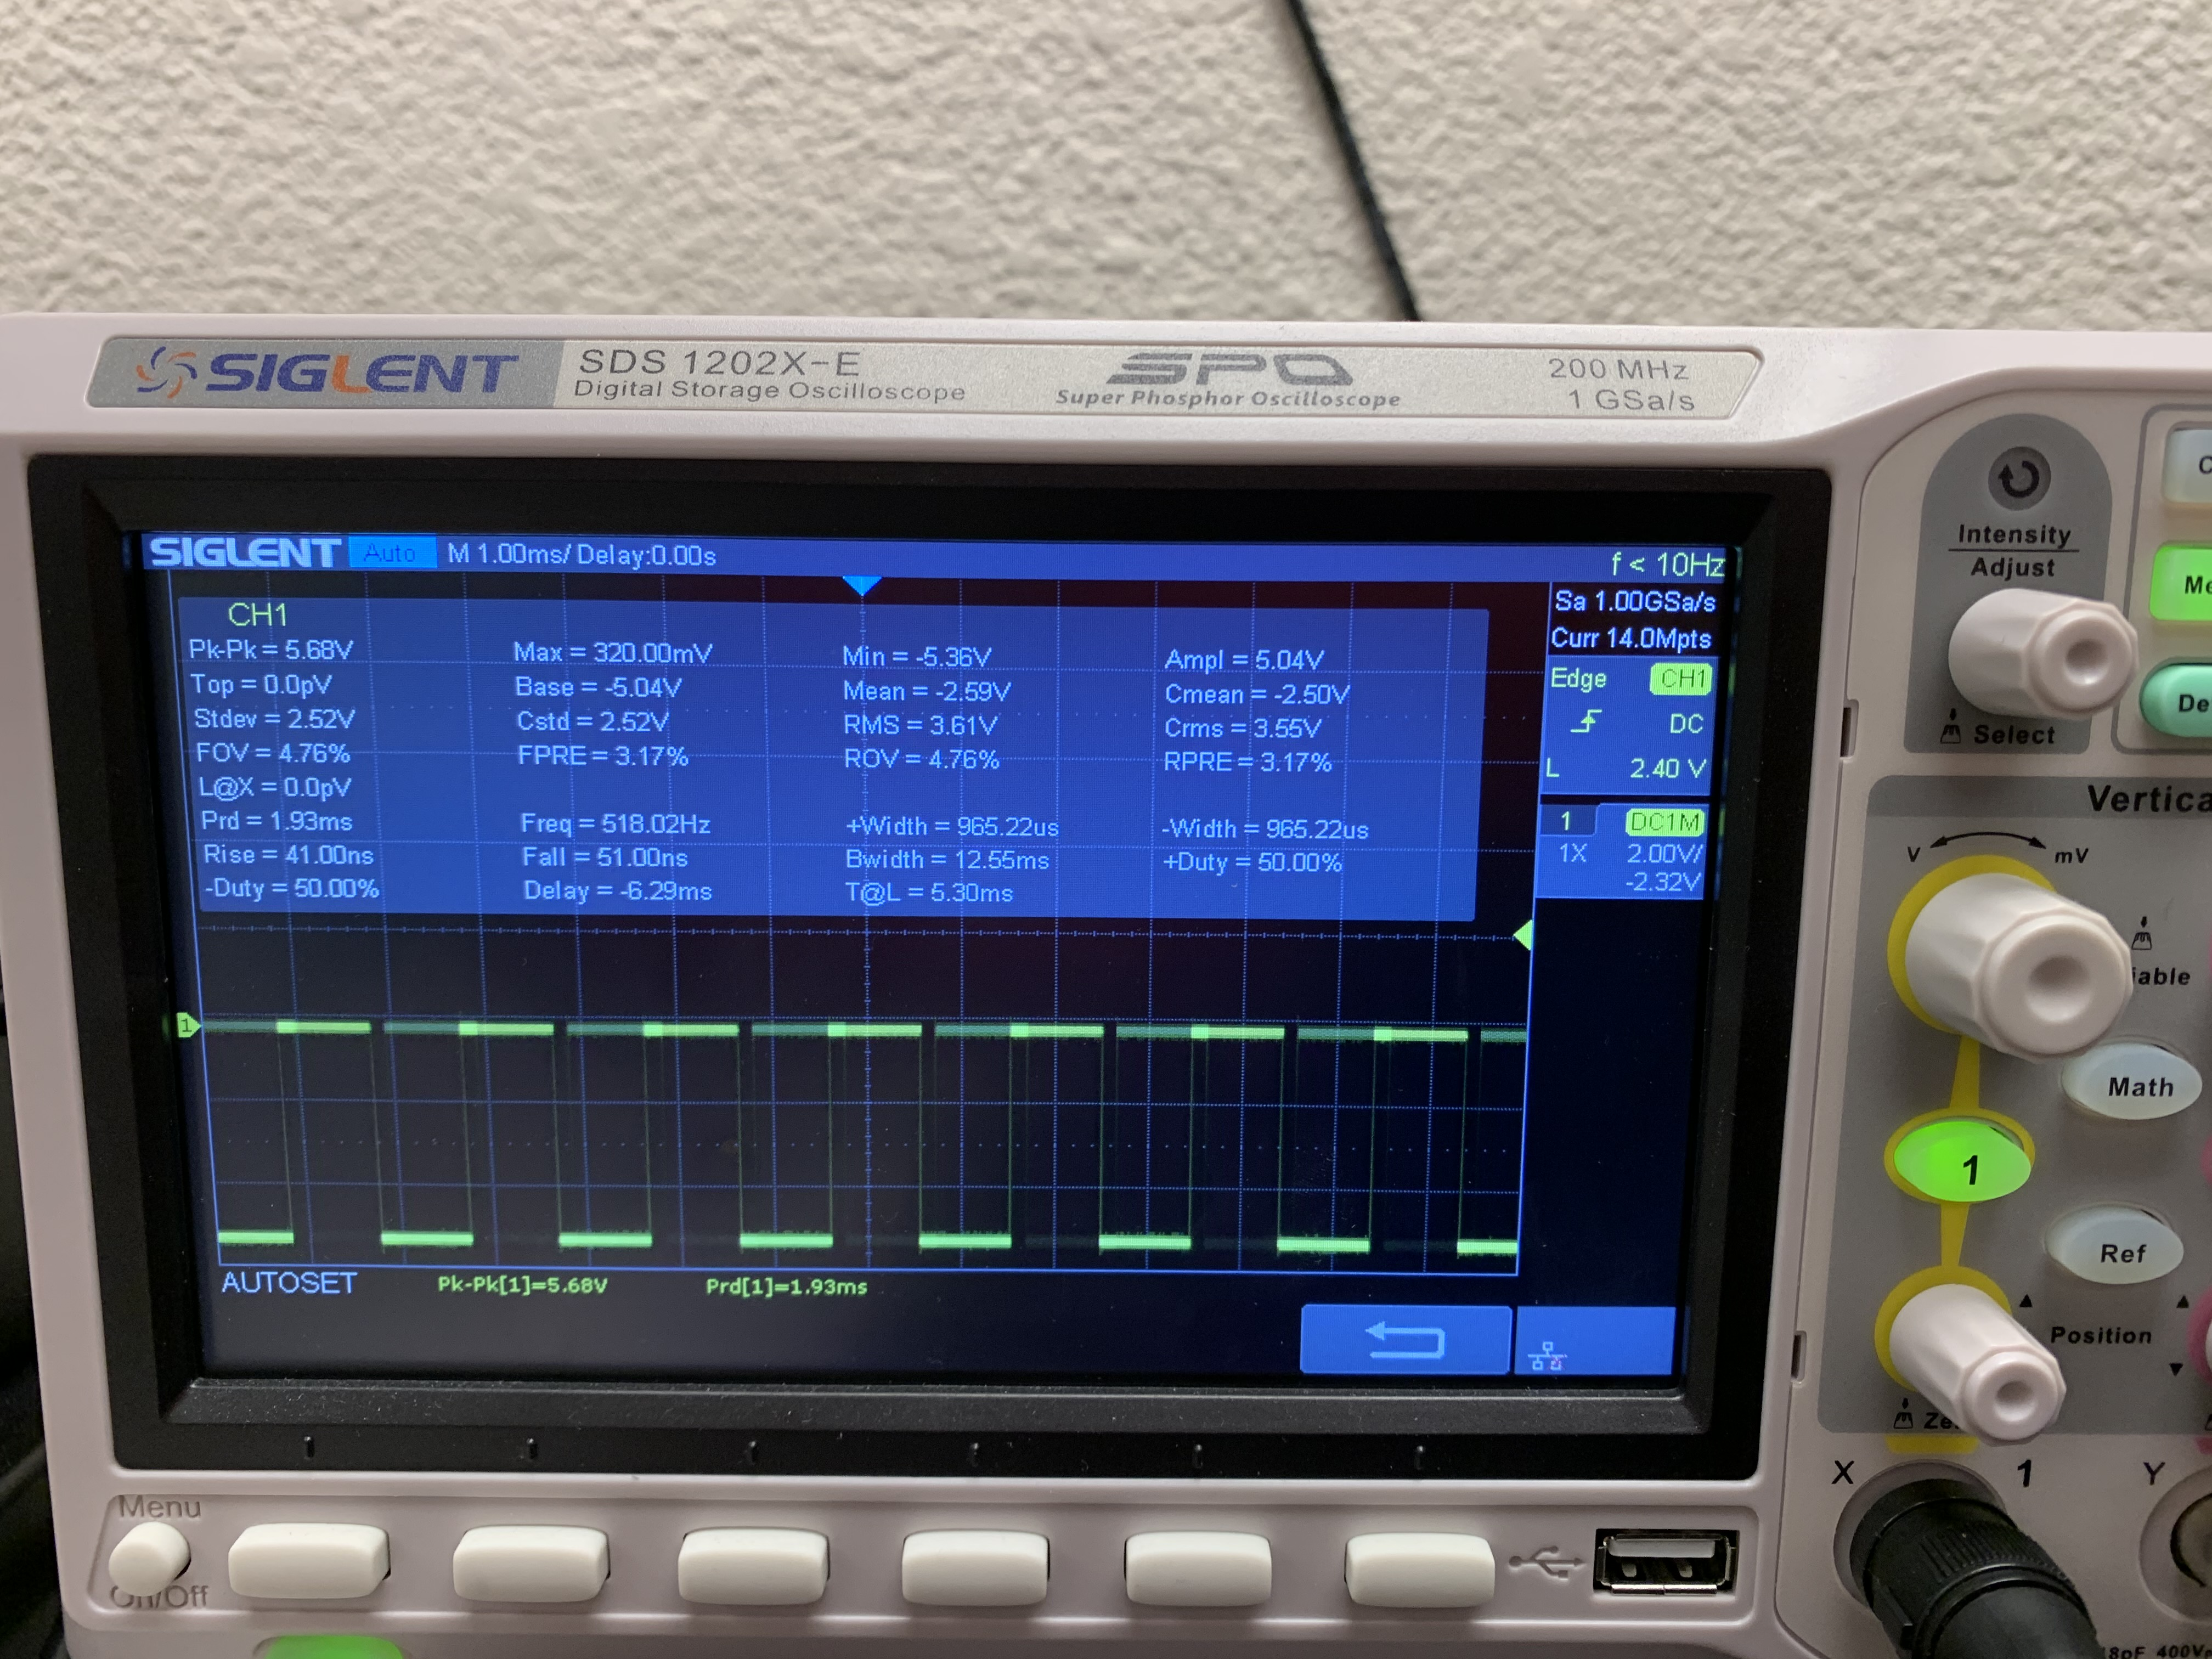
\includegraphics[scale=.05]{./images/2.jpg}\\
		\pagebreak
		Note: D\\
		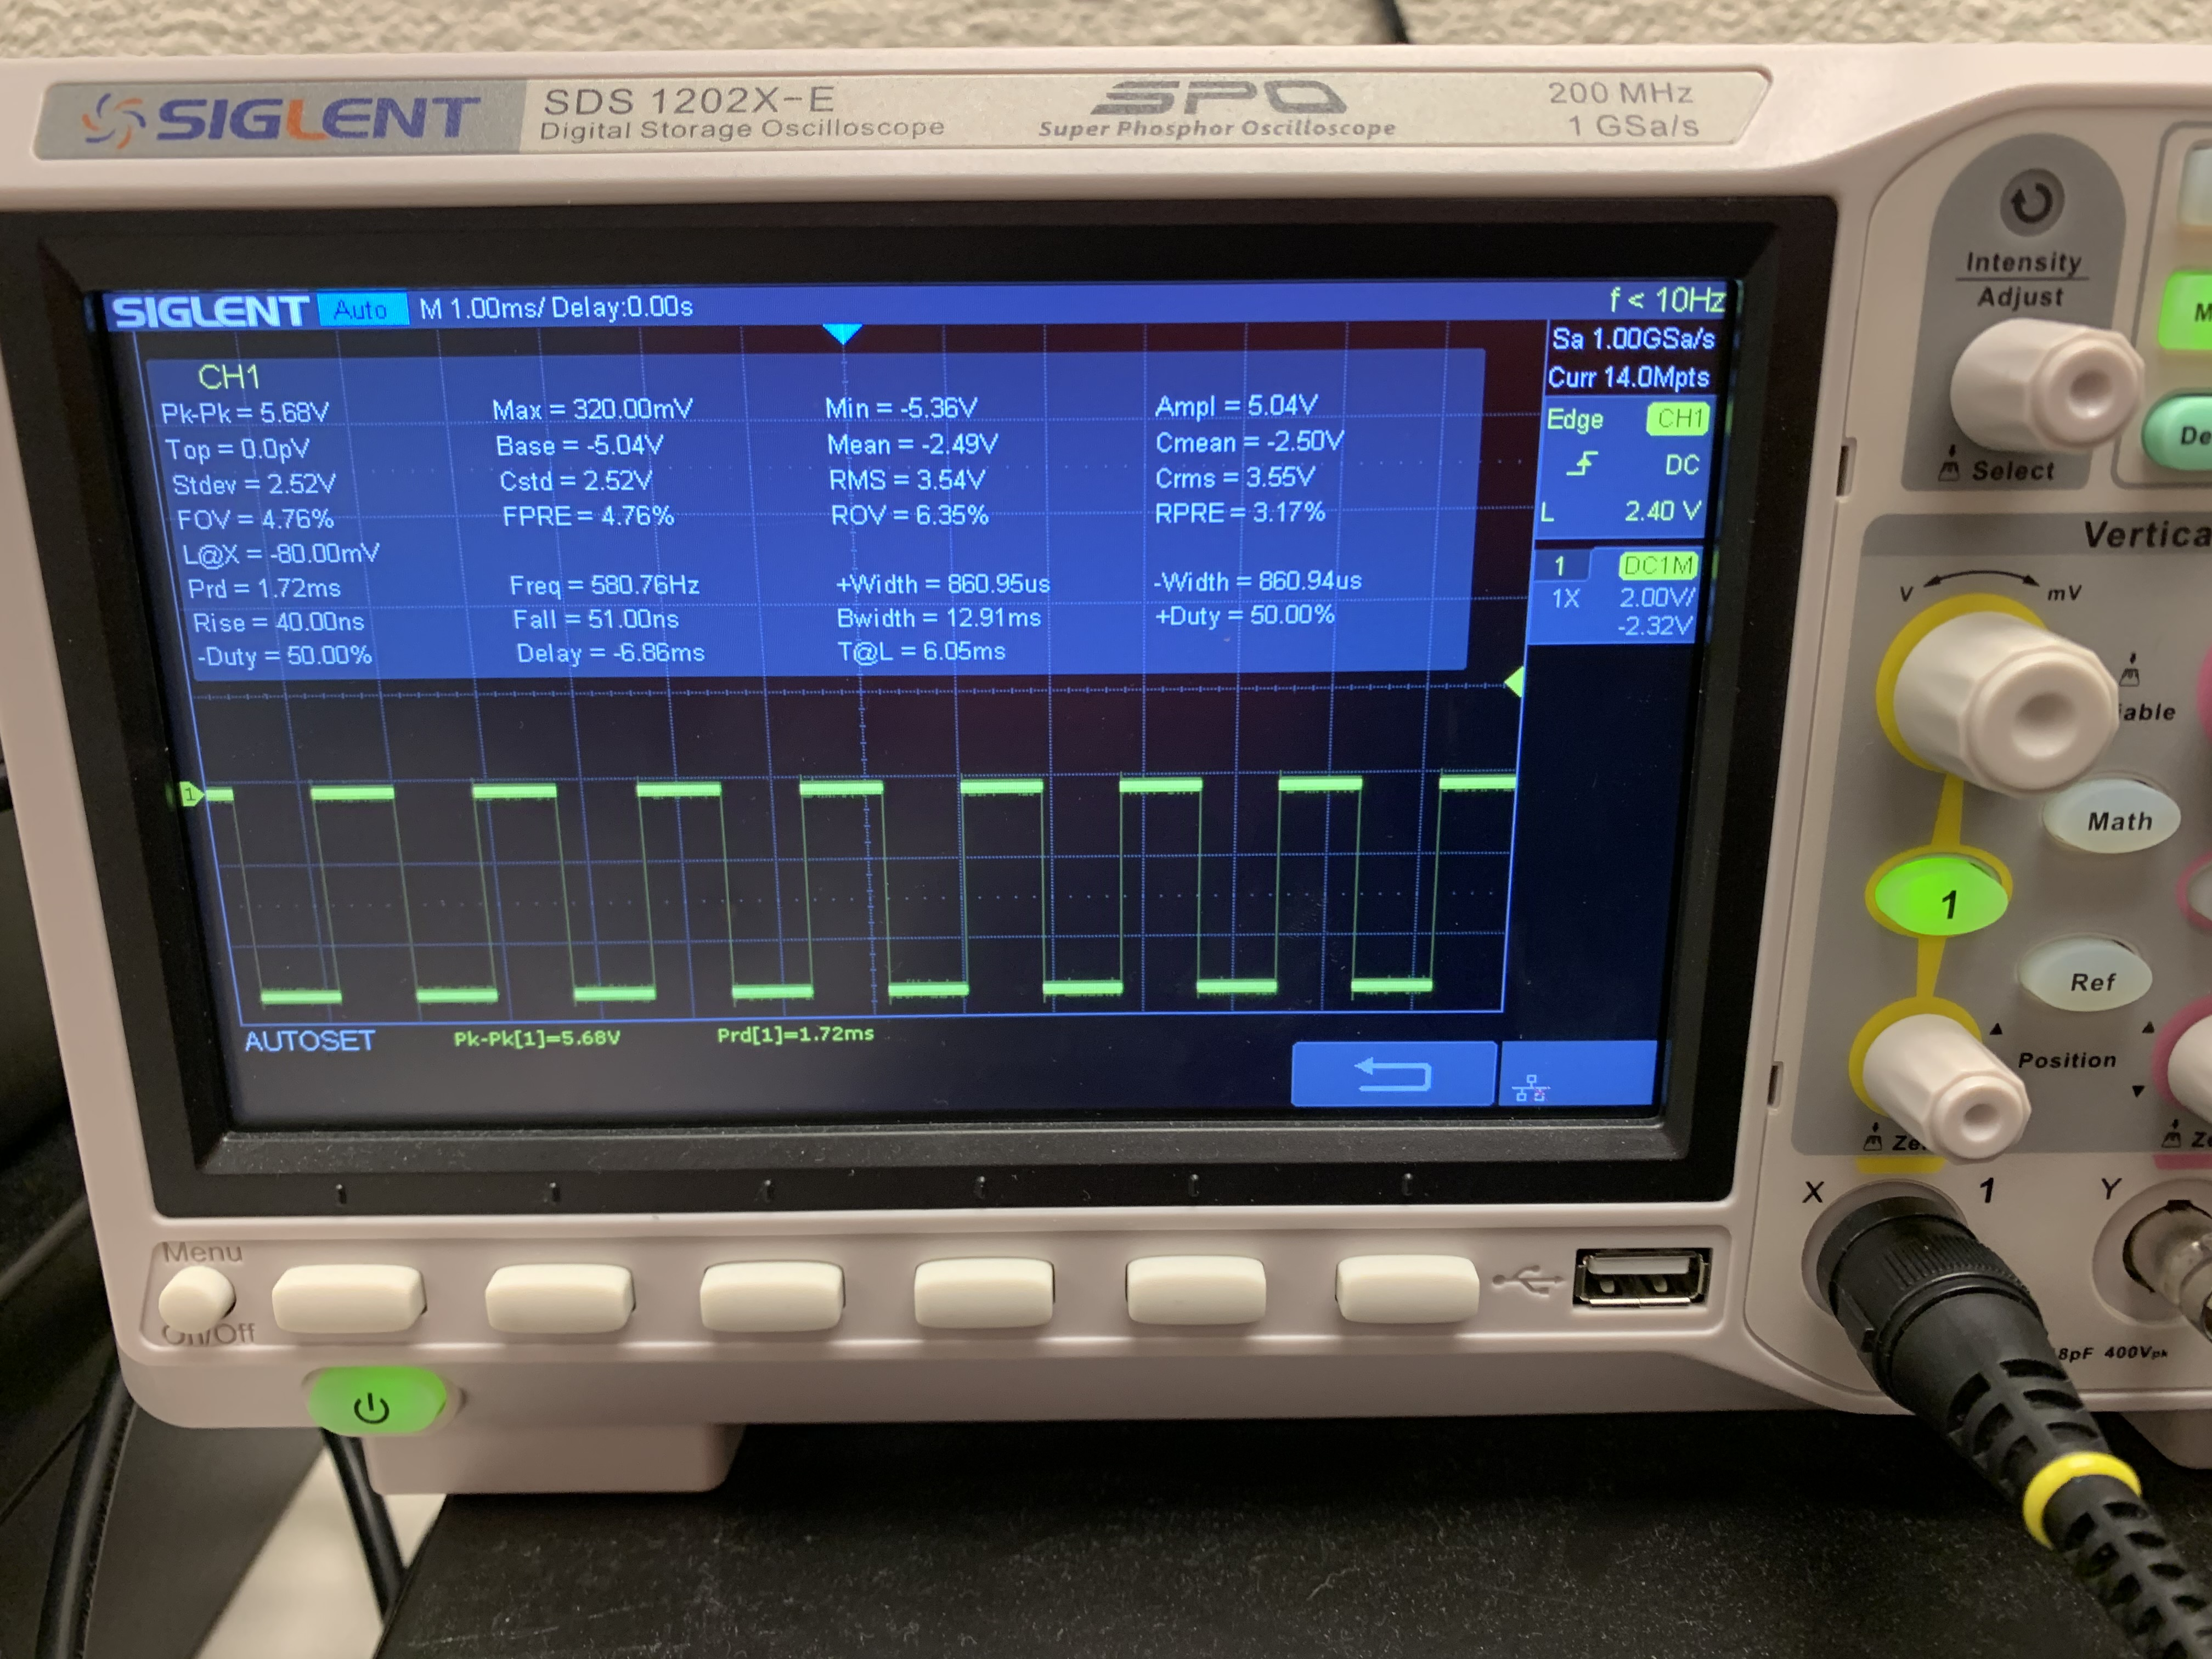
\includegraphics[scale=.05]{./images/3.jpg}\\
		Note: E\\
		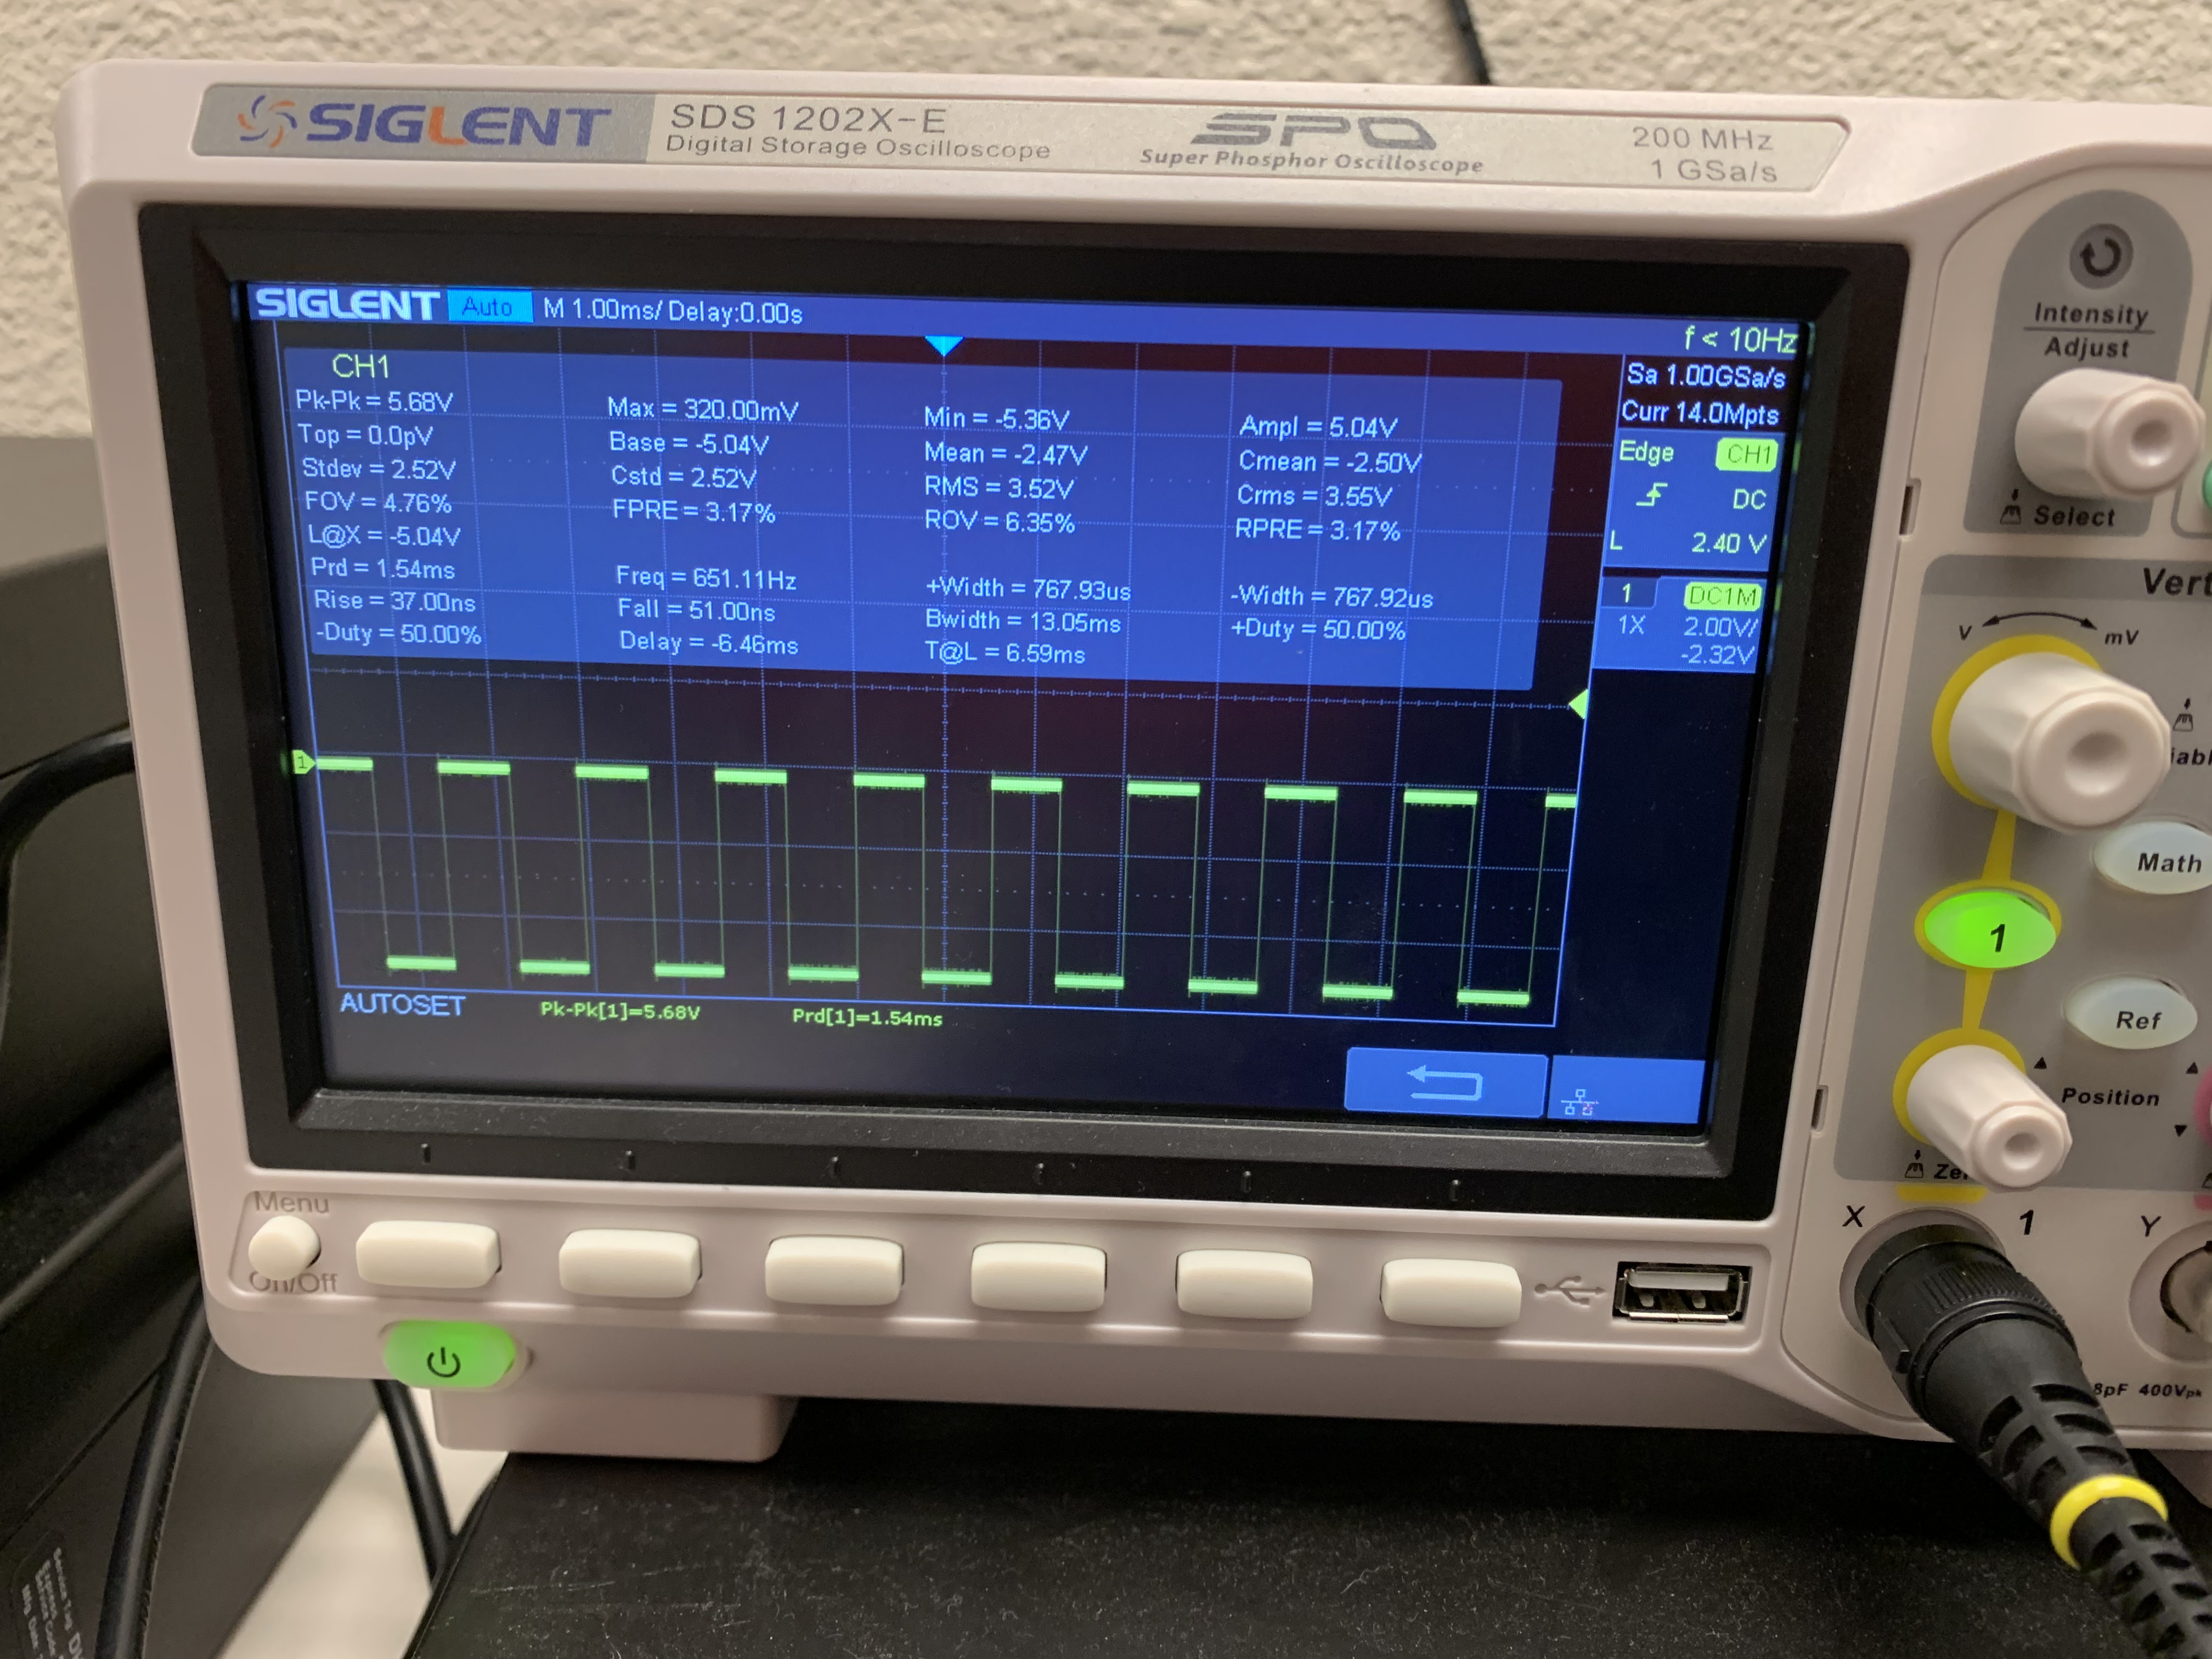
\includegraphics[scale=.05]{./images/4.jpg}\\
		Note: F\\
		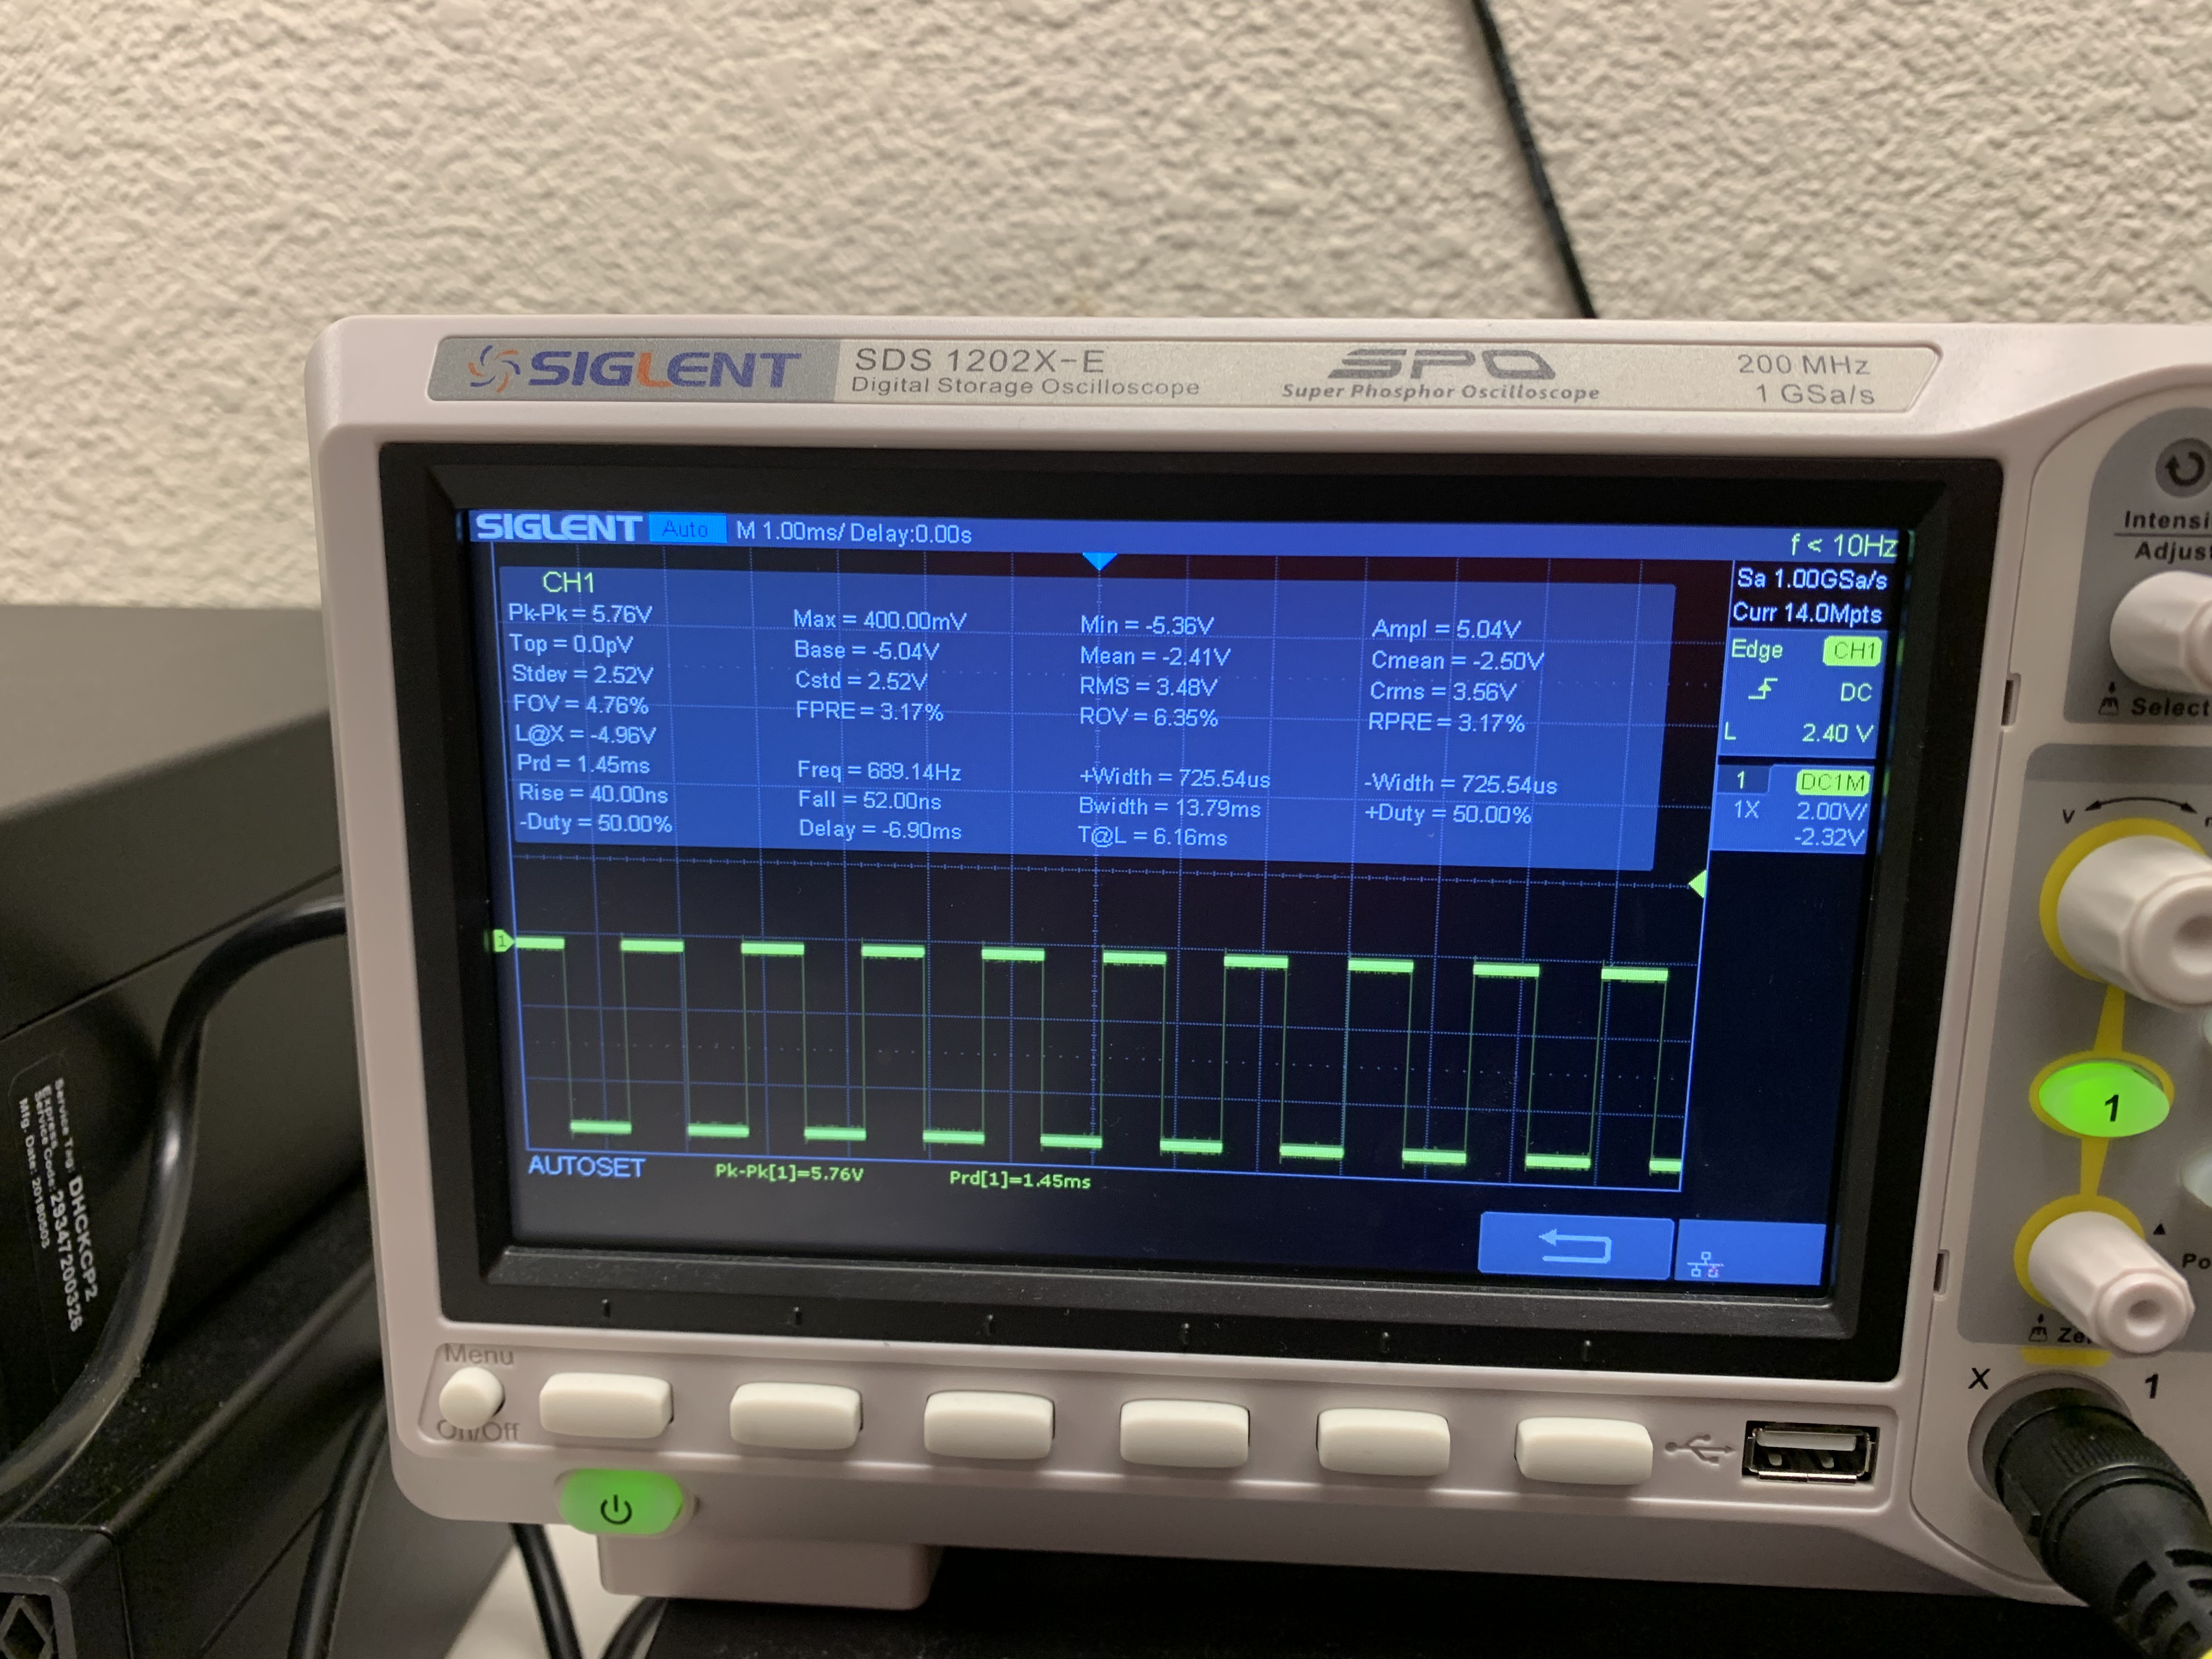
\includegraphics[scale=.05]{./images/5.jpg}\\
		\pagebreak
		Note: G\\
		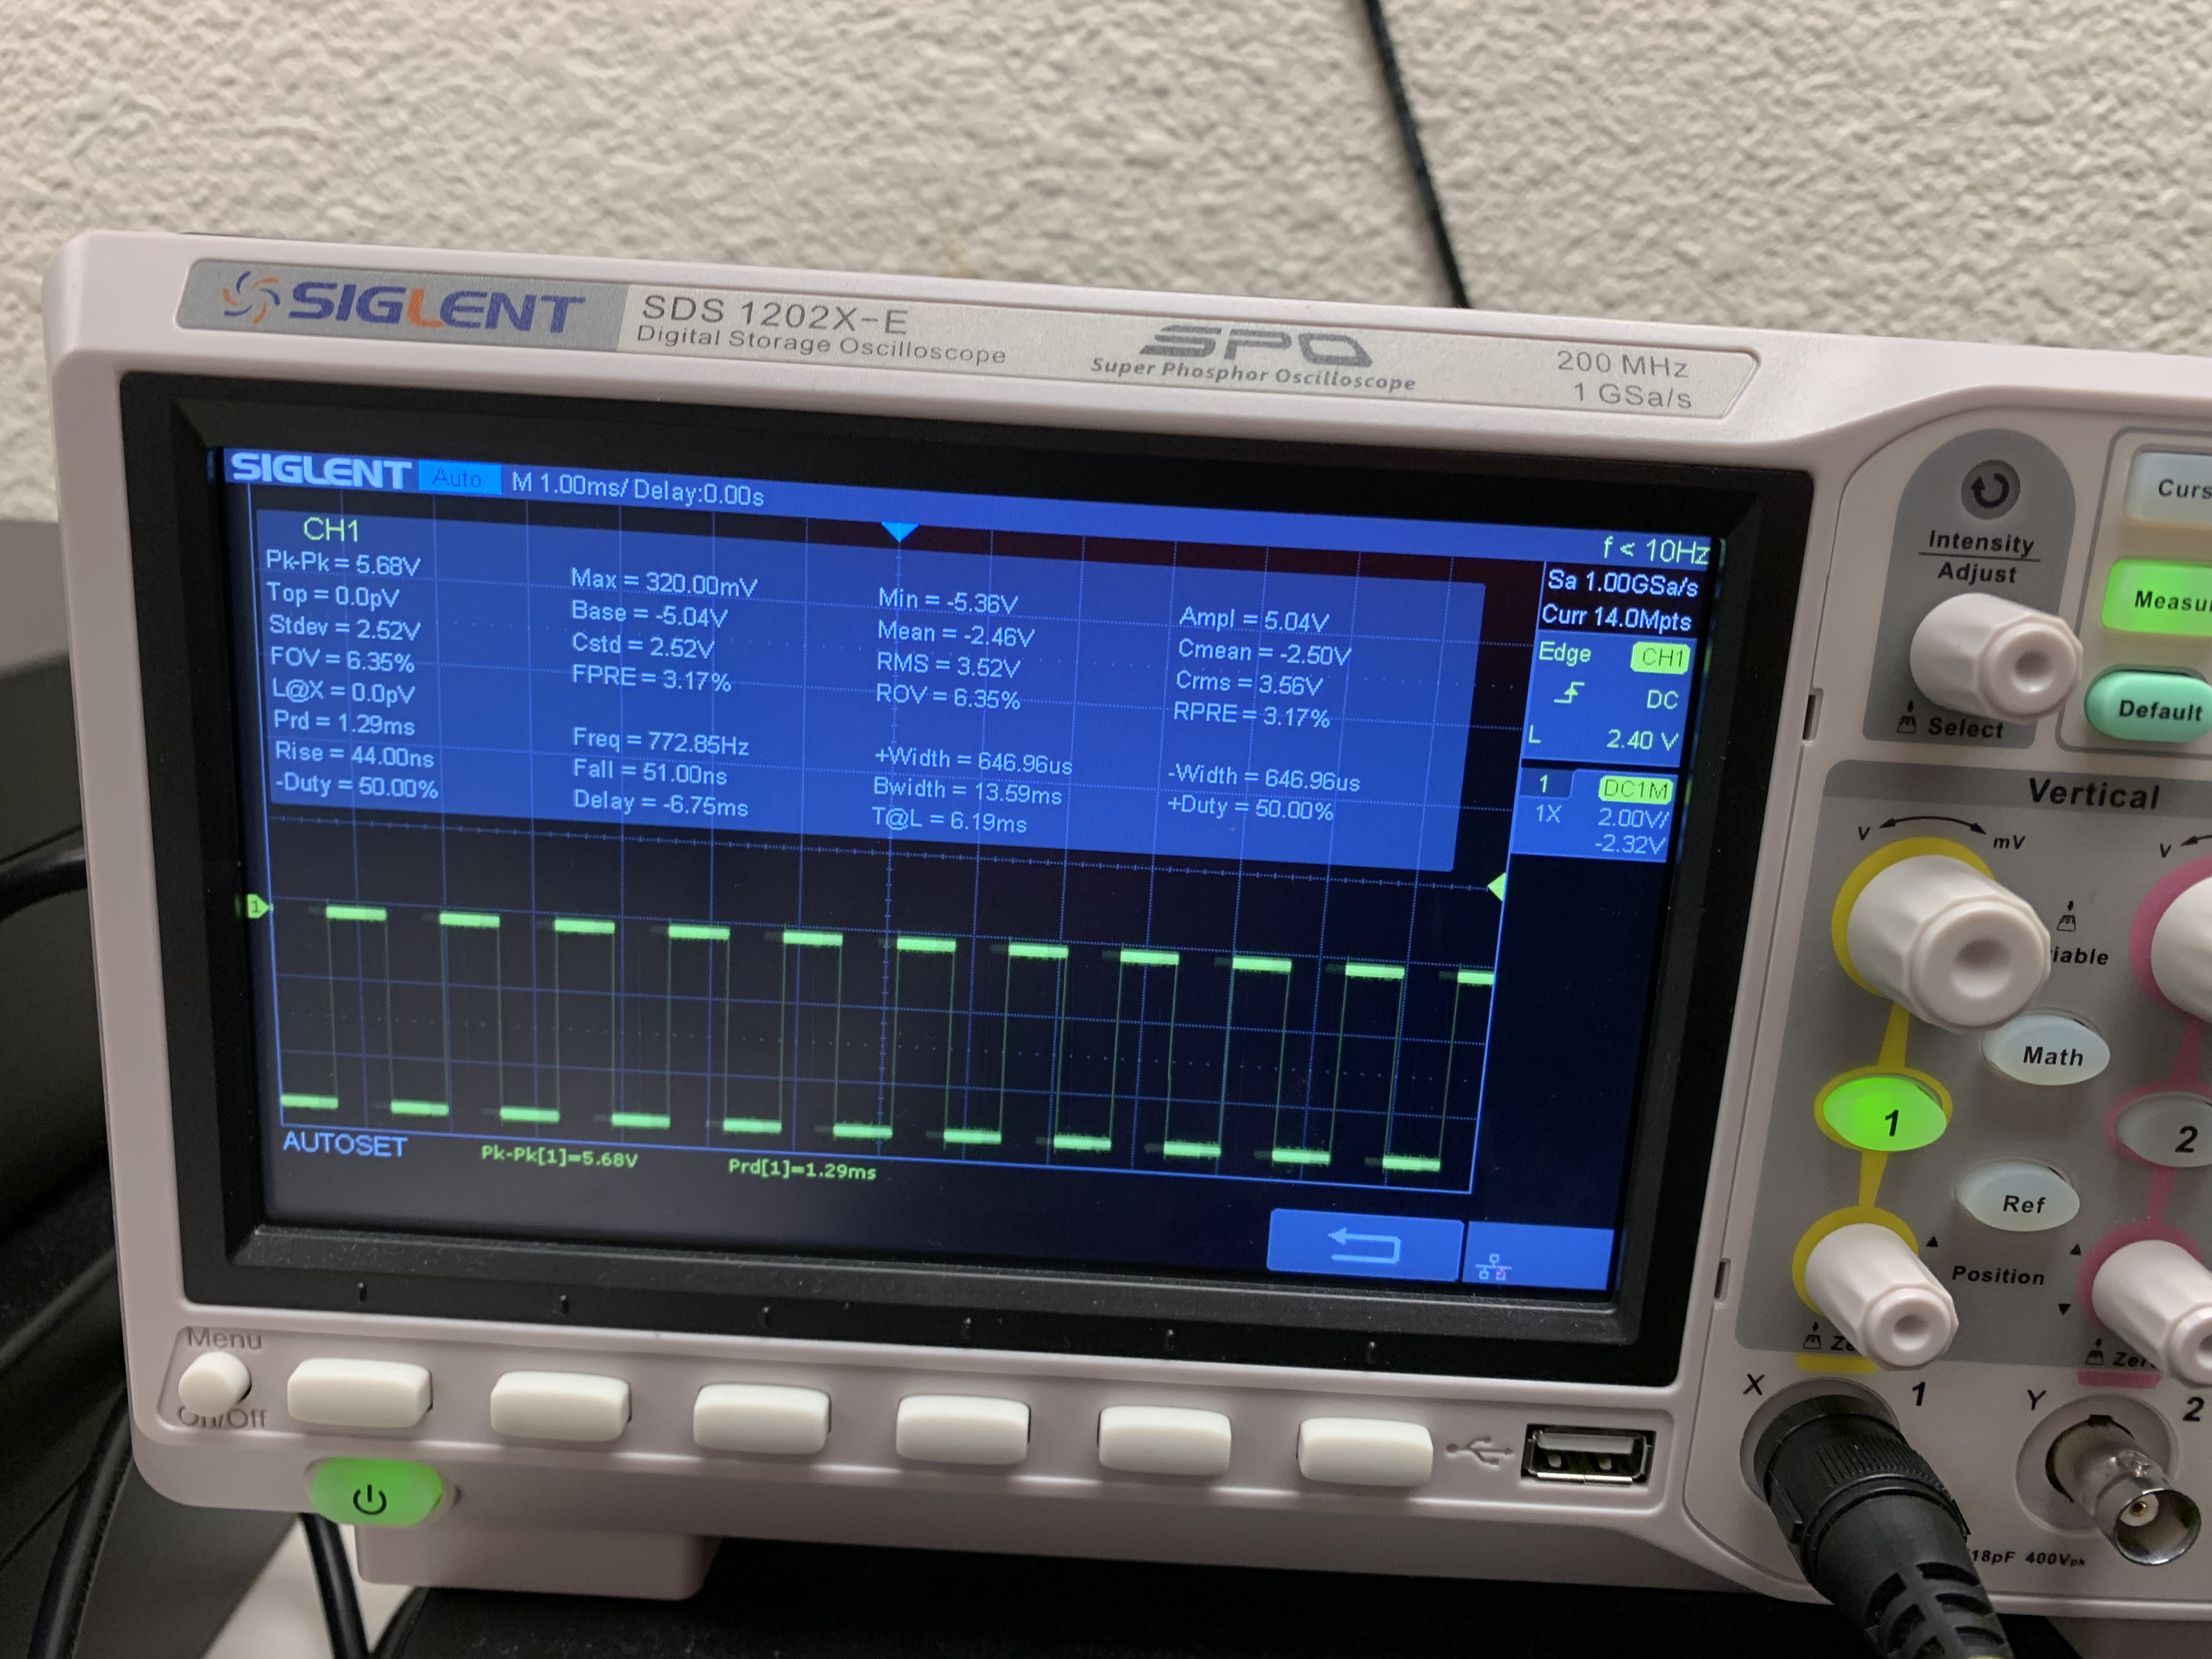
\includegraphics[scale=.05]{./images/6.jpg}\\
	\end{center}
	\pagebreak
	\lstinputlisting[language=C]{../src/main.c}
\end{document}
